\documentclass{beamer}

\usepackage[utf8]{inputenc}
\usepackage[T1]{fontenc}
\usepackage[french]{babel}
\usepackage{graphicx}
\usepackage{subcaption}
\usepackage{mathtools}

\title{Descripteur de textures}
\author{Kévin~\textsc{Bannier} \and Nicolas~\textsc{Laboureur} \and Amaury~\textsc{Louarn}}
\institute[ESIR]{%
    École Supérieure d'Ingénieurs de Rennes\\
    Université de Rennes 1
}

\begin{document}

\frame{\titlepage}

\begin{frame}
    \frametitle{Sommaire}
    \tableofcontents
\end{frame}

\section{Présentation}
\subsection{Motivations}
\begin{frame}
    \frametitle{Le descripteur de textures}
    \begin{block}{Utilité}
        Calcul de distances entre deux pixels en fonction de son environnement proche
    \end{block}
    \begin{exampleblock}{Exemple}
        \begin{figure}
            \centering
            \begin{subfigure}{0.3\textwidth}
                \centering
                
\includegraphics[height=2cm]{img/lena_texture1}
                \caption{}
            \end{subfigure}
            \begin{subfigure}{0.3\textwidth}
                \centering
                
\includegraphics[height=2cm]{img/lena_texture2}
                \caption{}
            \end{subfigure}
            \begin{subfigure}{0.3\textwidth}
                \centering
                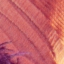
\includegraphics[height=2cm]{img/lena_texture3}
                \caption{}
            \end{subfigure}
        \end{figure}
    \end{exampleblock}
\end{frame}

\subsection{Fonctionnement}
\begin{frame}
    \frametitle{Vecteur d'attributs}
    Pour chaque pixel, on définit un vecteur d'attributs :
    \[
        z(x) =
        \begin{bmatrix}
            L &
            a &
            b &
            |\frac{\partial L}{\partial x}|&
            |\frac{\partial L}{\partial y}|&
            |\frac{\partial^2 L}{\partial x^2}|&
            |\frac{\partial^2 L}{\partial y^2}|&
            |\frac{\partial^2 L}{\partial x \partial y}|
        \end{bmatrix}^\top
    \]
    \vfill
    \begin{description}
        \item[$L$, $a$, et $b$ :] couleur du pixel (espace de couleur CIE*Lab)
        \item[$\frac{\partial L}{\partial x}$ et $\frac{\partial L}{\partial x}$ :] gradient de la luminance
        \item[$\frac{\partial^2 L}{\partial x^2}$, $\frac{\partial^2 L}{\partial y^2}$, et $\frac{\partial^2 L}{\partial x \partial y}$ :] dérivée seconde de la luminance
    \end{description}

    \vfill

    \begin{block}{Note}
        D'autres configurations sont possibles : utilisation de $R$, $G$ et $B$ {\tiny[Tuzet et al., 2006]}, utilisation de la position dans l'image : $x$ et $y$ {\tiny[Haracan et al., 2013]}.
    \end{block}
\end{frame}

\begin{frame}
    \frametitle{Matrice de covariance}
    La métrique utilisée permet de caractériser un seul pixel. Pour caractériser un patch de texture, on utilise la matrice de covariance des vecteurs d'attributs du patch :
    \[
        C_r (p) = \frac{1}{W} \sum_{q \in N_r^p} w_r (p, q) ( z(q) - \mu_r) {(z(q) - \mu_r)}^\top
    \]
    \begin{description}
        \item[$z(q)$ :] le vecteur d'attributs du pixel $q$
        \item[$\mu_r$ :] le vecteur moyen d'attributs des pixels du patch
        \item[$w_r$ :] terme de régularisation (poids des pixels en fonction de leur position dans le patch, un pixel au centre du patch aura plus d'importance qu'un pixel au bord)
        \item[$W$ :] facteur de normalisation $(W = \sum_{q \in N_r^p} w_r(p, q))$
    \end{description}
\end{frame}

\begin{frame}
    \frametitle{Mesure des distances}
    Les matrices de covariances ne sont pas dans un espace euclidien, il est donc difficile de faire des mesures de distances entre deux matrices de covariance.
    \vfill

    La décomposition de Cholesky permet de repasser dans un espace euclidien via une matrice triangulaire :
    \[
        \tiny \centering
        A =
        \begin{pmatrix}
            a_{1,1} & \cdots & a_{1,M} \\
            \vdots  & \ddots & \vdots  \\
            a_{N,1} & \cdots & a_{N,M} \\
        \end{pmatrix}
        =
        \begin{pmatrix}
            b_{1,1} & 0 & \cdots & 0 \\
            b_{2,1} & b_{2,2} & \cdots & 0 \\
            \vdots  & \vdots & \ddots & \vdots  \\
            b_{N,1} & b_{N,2} & \cdots & b_{N,M} \\
        \end{pmatrix}
        \times
        \begin{pmatrix}
            b_{1,1} & b_{2,1} & \cdots & b_{N,1} \\
            0       & b_{2,2} & \cdots & b_{N,2} \\
            \vdots  & \vdots  & \ddots & \vdots  \\
            0       & 0       & \cdots & b_{N,M}
        \end{pmatrix}
    \]

    On a alors un vecteur en métrique euclidienne :
    \[
        \begin{bmatrix}
            b_{1,1} &
            b_{2,1} &
            \cdots  &
            b_{2,2} &
            \cdots  &
            b_{N,M} &
        \end{bmatrix}
    \]
\end{frame}

\section{Objectifs}
\begin{frame}
    \frametitle{Objectifs}
    \begin{itemize}
        \item Décrire un pixel en fonction de son environnement proche
        \item Pouvoir calculer une distance entre deux textures
            \begin{itemize}
                \item càd la similarité entre pixels
            \end{itemize}
    \end{itemize}
\end{frame}

\section{Résultats}
\subsection{Carte des distances par rapport à un pixel}
\begin{frame}
    \frametitle{Carte des distances}
\end{frame}

\subsection{Patch match}
\begin{frame}
    \frametitle{Patch Match}
\end{frame}


\section*{Fin}
\begin{frame}
    \frametitle{Des questions~?}
\end{frame}

\end{document}
